\chapter{Conclusion}
la la la CUORE still needs more time to discover x...

\section{Future Prospects}
As shown in \autoref{fig:bolometer_mass_over_time}, CUORE is the latest experiment in a long line of experiments searching for \zeronubb~with a bolometric technique.
It is not the last, however, as another experiment, CUPID (CUORE Upgrade with Particle IDentification) is planned as the successor experiment to CUORE with expected sensitivity to \zeronubb~shown in \autoref{fig:cupid_lobster_plot}.
The main idea behind this upgrade is to add the ability to discriminate between $\alpha$ and $\gamma$ sources, which, as shown in \autoref{fig:cuore_background_budget}, greatly reduces the background contribution around the \zeronubb~Q-value from $\alpha$ particles that originate from detector and near surfaces.
In addition, a different isotope and bolometer is planned to be used, namely Li$_2\kern 0.1em^{100}$MoO$_4$, where $^{100}$Mo is now the parent isotope for \zeronubb~decays.
${^100}$Mo benefits as the isotope choice in this scenario since the Q-value for \zeronubb~decay is 3034 keV, far away from most $\gamma$ backgrounds \cite{Rahaman:2007ng}.
Naturally, a $^{100}$Mo parent would have higher-energy Majoron decays and the reductions in $\gamma$ backgrounds, paired with the $\alpha$ rejection, would reduce the backgrounds in this region considerably.
However, as the isotope choice is not yet finalized, even if CUPID does end up using $^{130}$Te crystals, Majoron searches will also benefit from this improvement.
In particular, one of the main possible backgrounds that strongly anticorrelates with the Majoron decays in CUORE is a contribution of $\alpha$ decays due to $^{147}$Sm from the surface of the copper frames, as shown in \color{red}refer to plot here\color{black}.

\begin{figure}
    \centering
    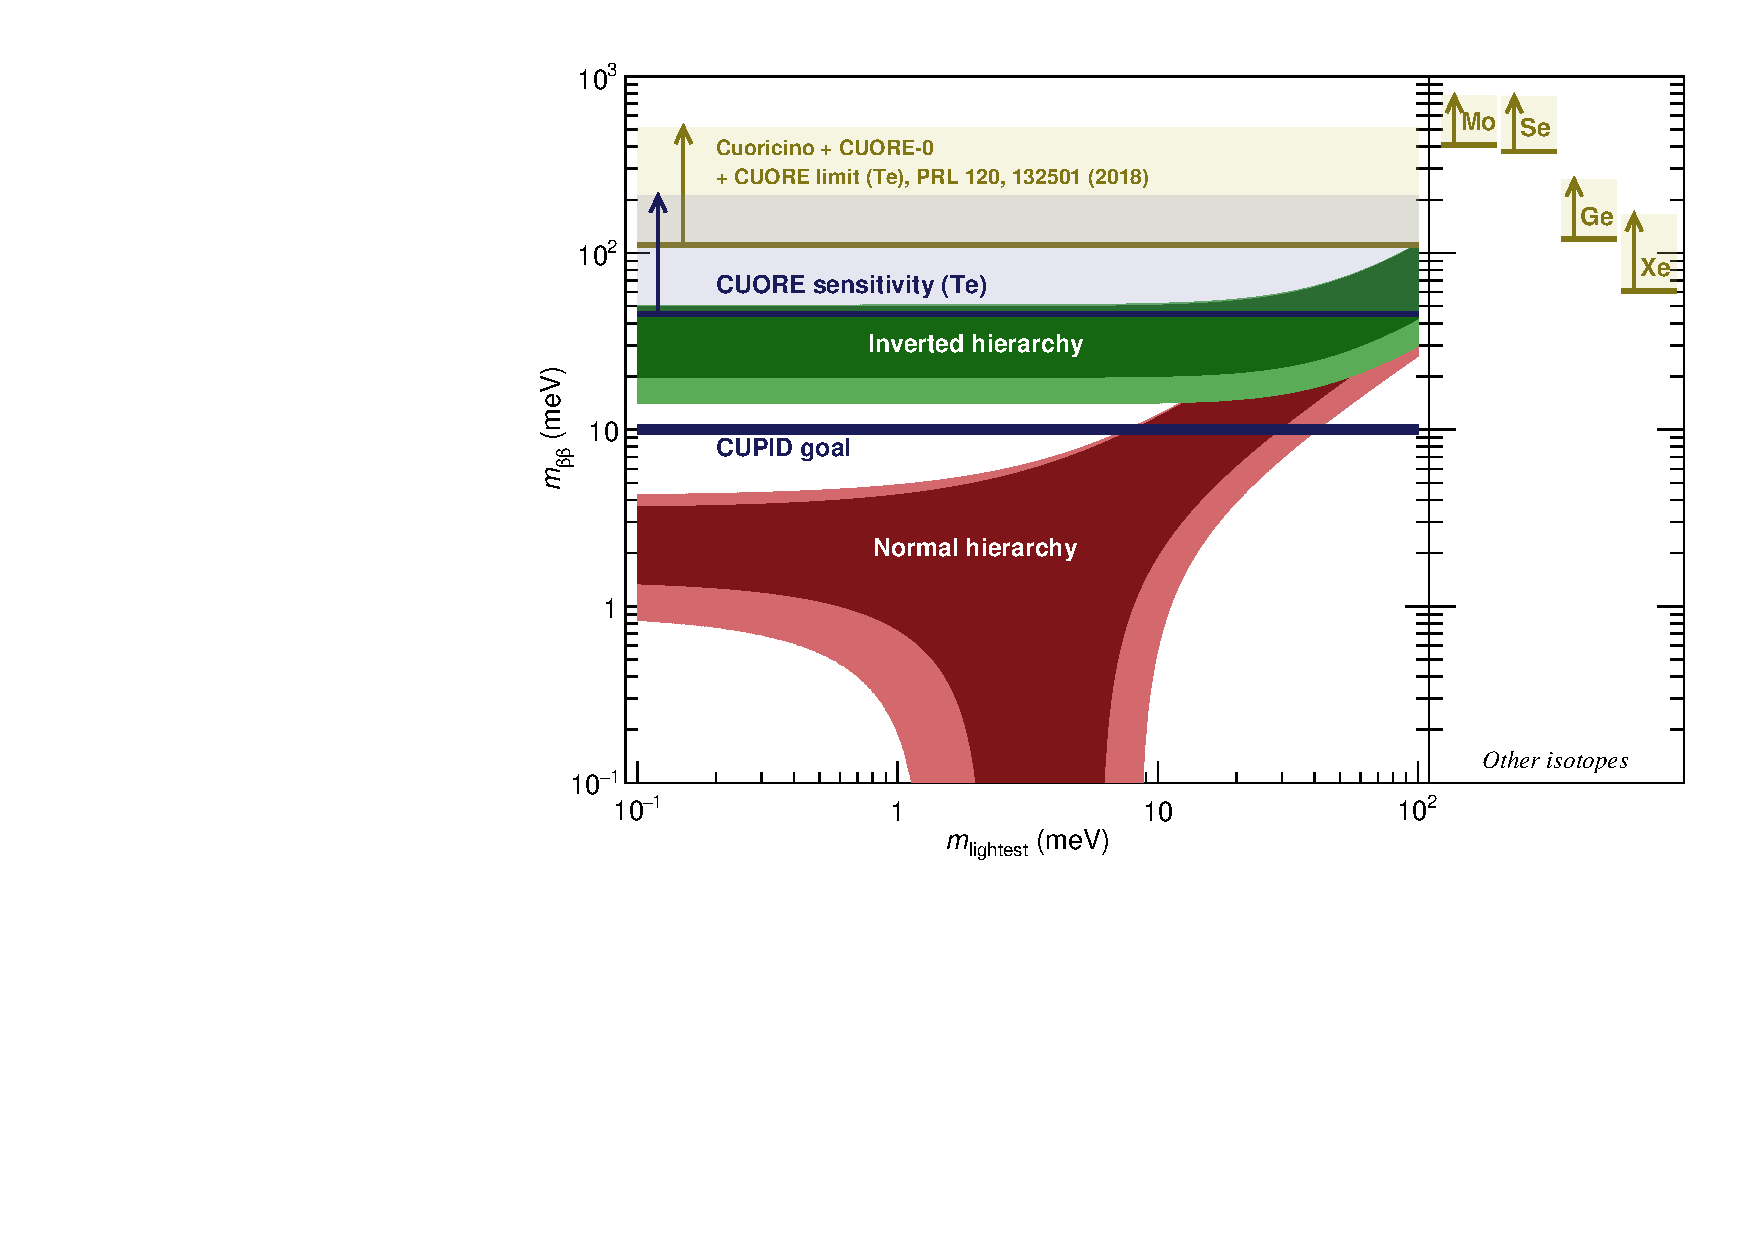
\includegraphics[width=0.8\linewidth]{Figures/Lobster_plot_cupid_mlightest_CL.pdf}
    \caption[The expected sensitivity for CUPID to \zeronubb]{The expected sensitivity for CUPID to \zeronubb.
    While the best limits and sensitivities of the current generation of experiments does not yet reach fully into the parameter space for the inverted hierarchy neutrino mass ordering, CUPID seeks to fully explore the space at 90\% C.L. While CUPID cannot make the same complete search in the parameter space for normal mass ordering, a significant proportion of the space will be excluded.}
    \label{fig:cupid_lobster_plot}
\end{figure}
